\chapter{Passivity}
\section{Outline}
Passivity is a concept related to energy dissipation or preservation. Informally we say that a system is passive if it doesn't produce energy internally. Energy plays a fundamental role and represent a sort of common unifying language across all physical domains. Most physical systems have common I/O characteristics dictated by energy conservation, transportation, dissipation.
Not surprisingly passivity-like concepts are common to various scientific domains: Physics, Electronics, Control.
\section{Passive dynamical system}
We will consider systems with the following structure:
\[
S:\begin{cases}
	&\dot{x}(t)=f(x(t),u(t)), \qquad x(0)=x_0 \in \Re^n\\
	&y(t)=g(x(t),u(t))
\end{cases}\qquad
\text{with }f(0,0)=0 \qquad g(0,0)=0.
\]
Let's introduce now a formal definition
\begin{defn}[Passive dynamical system]
	System S is passive if there exists a function $V(\cdot)\colon\Re^n\to\Re$ semipositive definite and continuously differentiable, called \emph{storage function}, such that:
	\[
	uy\ge\frac{\delta V}{\delta x}(x)f(x,u)+\epsilon u^2+\delta y^2+\rho\phi(x).\qquad \forall(x,u)\in \Re^n\times\Re)
	\]with $\epsilon,\delta,\rho\in\Re^+$ and $\phi(\cdot)$ positive definite.
\end{defn}
In particular, system S is:
\begin{itemize}
	\item \emph{strictly passive w.r.t. the input if $\epsilon >0$}
	\item \emph{strictly passive w.r.t. the output if $\delta >0$}
	\item \emph{strictly passive w.r.t. the state if $\rho >0$} 
\end{itemize}
We can now give to the definition a physical interpretation:
\begin{itemize}
	\item the storage function $V(\cdot)$ represents the \underline{internal stored energy};
	\item the supply rate \emph{uy} is the \underline{power exchanged with the external world}.
\end{itemize}
By taking the integral of $uy\ge\frac{\delta V}{\delta x}(x)f(x,u)$ we get the \emph{basic passivity condition}:
\[
V(x(t))\le V(x(0))+\int_{0}^{t}u(s)y(s)ds
\]which can be interpreted as follows: the current internal energy is at most equal to the initial energy plus some energy supplied from outside. Which is equivalent to say that there is ''no internal generation of energy''. If the system is passive the total energy at time t is less then the original plus the external one.
\section{Example: RLC circuit}
Let's make now an example of a passive physical dynamical system: the RLC circuit.
\begin{figure}[H]
	\centering
	\includegraphics[scale=0.4]{immagini/RLC}
	\caption{RLC circuit}
	\label{fig:rlc}
\end{figure}
We consider as the input the voltage \emph{u}, as the output the current \emph{y}, and as states variables the current in the inductor $(x_1)$ and the voltage on the capacitor $(x_2)$. Thanks to the Kirchhoff laws:
\[
\begin{cases}
	 L\dot{x}_1=u-R_2x_1-x_2\\
	C\dot{x}_2=x_1-\frac{1}{R_3}x_2\\
	y=x_1+\frac{1}{R_1}u
\end{cases}
\]
The energy stored in the circuit (storage function):\[V(x)=\frac{1}{2}Lx_1^2+\frac{1}{2}Cx_2^2\]
Its derivative along the trajectories of the system is given by
\[
\begin{aligned}
	\dot{V}(x)&=Lx_1\dot{x}_1+Cx_2\dot{x}_2\Rightarrow x_1(u-R_2x1-x_2)+x_2(x_1-\frac{1}{R_3}x_2) \\
	&=ux_1-R_"x_1^2-\frac{1}{R_3}x_2^2=uy-\frac{1}{R_1}u^2-R_2x_1^2-\frac{1}{R_3}x_2^2.
\end{aligned}
\]
Not surprisingly we have:
\[
\dot{V}(x)\le uy
\]
that is the power stored in the RLC circuit is smaller than or equal to the power provided at its input (it is passive, with no energy generators). From which it follows \[
V(x(t))-V(x(0))\le\int_{0}^{t}u(s)y(s)ds
\]
That is the increment of the stored energy cannot exceed the amount of energy absorbed by the circuit in the same time interval. The difference is the energy dissipated by the resistors.
\\Recalling the storage function differentiated along the trajectories of the system $\dot{V}(x)=uy-\frac{1}{R_1}u^2-R_2x_1^2-\frac{1}{R_3}x_2^2$ we will analyze four different case to explain different sort of passivity:
\paragraph{1) $R_1=R_3=\infty; R_2=0 $}
In this case the passivity condition reduces to \[uy=\dot{V}(x)\] since there is no energy dissipation because the internal energy is equal to the feeded to the system, the system is \textcolor{red}{conservative}.
\paragraph{2) $R_3=\infty; R_2=0$} In this case the passivity condition reduces to \[uy=\dot{V}(x)-\frac{1}{R_1}u^2\] and dissipation rate proportional to the square of u. So the system is \textcolor{red}{strictly passive with respect to the input}.
\paragraph{3) $R_1=R_3=\infty$} In this case the passivity condition is \[uy=\dot{V}(x)+R_2x_1^2=\dot{V}(x)+R_2y^2\] so since the dissipation rate is proportional to the square of y, the system is \textcolor{red}{strictly passive with respect to the output}.
\paragraph{4) $R_1=\infty$} In this case the passivity condition is \[uy=\dot{V}(x)+R_2x_1^2+\frac{1}{R_3}x_2^2=\dot{V}(x)+R_2y^2.\] The dissipation rate is a positive function of x $\phi(x)\colon=R_2x_1^2-\frac{1}{R_3}$ so the system is \textcolor{red}{strictly passive with respect to the state variables}.
\section{Passivity for static systems}
The notion of passivity extends also for static systems.\\
Given a system $S:\qquad y(t)=g(u(t))$
\begin{defn}[Static passive system]
	A system S is passive if there exists, $\epsilon,\gamma \in \Re^+$ such that: \[uy \ge\epsilon u^2+\gamma y^2, \forall u \in \Re\]
	In particular, system  S is:
	\begin{itemize}
		\item[-] \emph{strictly passive w.r.t.the input if $\epsilon>0$}
		\item[-] \emph{strictly passive w.r.t. the output if $\gamma>0$}
	\end{itemize} 
\end{defn} 
From this definition we can notice that since the righten part of the equation is a sum of positive terms if the system is passive, the "power" flowing into the system is never negative ($uy\ge 0$). Furthermore the system does not produce energy, it can only absorb or dissipate. A typical example can be the electrical resistance $y=Ru$ which dissipates energy since the power flow is $uy=Ru^2\ge 0$.
\subsection{Characterization in terms of a sector}
Given a static function how can we immediately understand if it is passive or not? Since for the definition we have to multiply the output for the input passivity imposes a constraint in the graph of the static function. The function must lie in the first and third quadrant since $uy\ge ug(u)\ge 0$ as we can see in \ref{fig:sfunc}. This is can interpreted as a sector with $[0,\infty]$ bounds.
\begin{figure}[H]
	\centering
	\begin{subfigure}[b]{0.3\textwidth}
		\centering
		\includegraphics[scale=0.25]{immagini/staticpassive system}
		\caption{Static function}
		\label{fig:sfunc}
	\end{subfigure}
	\hfill
	\begin{subfigure}[b]{0.3\textwidth}
		\centering
		\includegraphics[scale=0.25]{immagini/static passive sector}
		\caption{Sector}
		\label{fig:sectpass}
	\end{subfigure}
	\hfill
	\label{fig:staticpass}
	\caption[]{}
\end{figure}
We now want to give a different but equivalent characterization of the previous definition in terms of a sector as showed in \ref{fig:sectpass}.
\paragraph{Equivalent characterization} The condition $\exists  \epsilon,\gamma\in \Re^+\colon uy \ge \epsilon u^2+\gamma y^2 \forall u \in \Re$ is equivalent to say that $g(\cdot)$ is within a sector in the first and third quadrant. We can formulate the concept of sector more formally exploiting the definition of sector as:
\[
\exists k_1,k_2 \qquad 0\le k_1\\le k_2 \le \infty \colon (y-k_1u)(k_2u-y)\ge0, \forall u \in \Re.
\]
\section{Sufficient conditions for passivity}
\subsection{Asymptotically stable linear dynamical systems}
As introduction let's make an example on linear dynamical systems and its relation to the concept of passivity. Let's consider a minimal representation of such a system.
\[\begin{cases} 
	\dot{x}(t)=Ax(t)+Bu(t),\qquad x(0)=x_0\in\Re^n\\
	y(t)=Cx(t)\\
\end{cases}
\] with: $Re[\lambda_i(A)]<0, i=1,2,\dots,n$ and (A,B) reachable and (A,C) observable such that $G(s)=C(sI-A)^{-1}B+D$. In particular:
\begin{prop}
	If G(s) is strictly positive real, then, S is strictly passive w.r.t. the state.
\end{prop}
\begin{prop}
	If G(s) is positive real, then, S is passive.
\end{prop}
But what does it mean positive or strictly positive transfer function?
\begin{defn} [Positive real]
	A transfer function G(s) with all poles in the open left-hand side plane is \textcolor{red}{positive real} if $Re[G(j\omega)] \ge0, \forall  \omega \ge 0$
\end{defn}
\begin{defn} [Strictly positive real]
	A transfer function G(s) with all poles in the open left-hand side plane is \textcolor{red}{strictly positive real} if $G(s-\epsilon)$ is positive real for some $\epsilon$.
\end{defn}
We will see now a characterization of strictly positive realness through \textbf{positive real lemma}.
\paragraph{Positive real lemma}
The transfer function $G(s)=C(sI-A)^{-1}B+D$ of a reachable, observable, and asymptotically stable system is \emph{strictly positive real} if and only if there exist:
\begin{itemize}
	\item an nxn matrix P symmetric and positive definite
	\item a nx1 vector L
	\item a constant $\omega$
\end{itemize}
such that: \qquad
\boxed{
\begin{aligned}
	&PA+A'P=-LL'-\epsilon P\\
	&PB-C'=-\omega L\\
	&2D=\omega^2
\end{aligned}
}
\\
And this is also valid for simply positive realness but with $\epsilon$ equal to 0.
\\
Using this lemma we can prove the first proposition of this section which states: \emph{if G(s) is strictly positive real, then, S is strictly passive w.r.t. the state.} In order to prove the prove the proposition we have to introduce a storage function that recall us the candidate Lyapunov function used to prove stability
\begin{proof}
	Candidate storage function: $V(x)=\frac{1}{2}x'Px$. P is guaranteed to exist thanks to the positive real lemma since G(s) is strictly positive real. So we now that V(x) is symmetric and positive definite and in consequence is a good candidate storage function.
	Now we check if the passivity inequality is satisfied and in order to do it we take the derivative of V(x).
\[
	\begin{aligned}
		uy-\frac{\delta V}{\delta x}(x)f(x,u)&=uCx+Du^2-\frac{1}{2}x'(PA+A'P)x-x'PBu\\
		&=u(B'P+\omega L')x+\frac{1}{2}(\omega^2u^2+x'LL'x+\epsilon x'Px)-uB'Px\\
		&=\frac{1}{2}\left( (L'x+\omega u)^2+\epsilon x'Px\right) \ge \frac{1}{2}\epsilon x'Px, \forall(x,u)\in \Re^n \times \Re
	\end{aligned}
\]
\end{proof}
For the other proposition (positive realness) the proof is equivalent but $\epsilon$ is equal to 0 so we get: \[uy\ge \frac{\delta V}{\delta x}(x)f(x,u)\]
\subsection{Nonlinear dynamical systems affine in the input} 
First of all we define the concept of ''affine'' function: \\ an \textbf{affine} function of a certain quantity is affine in that quantity if is of the form e.g $\gamma(\delta)=\delta\cdot const+const$


\[\text{S}: \begin{cases}
\dot{x}(t)=\alpha(x(t))+\beta(x(t))u(t), \qquad x(0)=x_0\in\Re^n\\
y(t)=\gamma(x(t))
\end{cases}
\]
\begin{prop}
	If there exists V($\cdot$): $\Re^n \to \Re$ positive semidefinite and continuously differentiable function such that: \[\frac{\partial V}{\partial x}\alpha(x)\le -\delta \gamma^2, \qquad frac{\partial V}{\partial x}\beta(x) = \gamma, \forall x \in \Re^n\] for some $\delta\ge0$, then S is passive. If $\delta>0$, then S is strictly passive w.r.t the output.
\end{prop}
\begin{proof}
	\[
	\begin{aligned}
		uy-\frac{\partial V}{\partial x}(x)f(x,u)&=uy-\frac{\partial V}{\partial x}(x)()\alpha(x)+\beta(x)u)\\
		&=u\gamma-\frac{\partial V}{\partial x}(x)\alpha(x)-\gamma(x)u\\
		&=-\frac{\partial V}{\partial x}\alpha(x)\ge \delta\gamma^2(x)=\delta y^2, \forall(x,u)\in\Re^n\times\Re
	\end{aligned}
	\]
\end{proof}
But now we ask ourself why is passivity important in control? Because we show that there is a strong relation between passivity and stability of the zero equilibrium with zero input. Also a passive system is ''easily stabilizable'' form the output and a system can be made passive by choosing the right output. Furthermore proper interconnections of passive systems are passive.
\subsubsection{Passivity \& stability of the equilibrium}
\begin{thm}
	If a dynamical system S is \underline{passive with positive definite storage function}, then, x=0 is a (Lyapunov) stable equilibrium for the system \underline{with zero input}.
\end{thm}
\begin{proof}
	Let use the storage function as candidate Lyapunov function. \\If S is passive and u=0, then $\dot{V}(\cdot)$ is negative semidefinte, since from \[
	uy\ge\frac{\partial V}{\partial x}(x)f(x,u)+\epsilon u^2+\gamma y^2+\rho\phi(x),\forall(x,u)\in \Re^n\times\Re
	\] we get \[\dot{V}(x)=\frac{\partial V}{\partial x}(x)f(x,\underline{0})\le-\gamma y^2-\rho \phi(x),\forall x \in \Re^n\]
\end{proof}
\begin{thm}
	If a dynamical system S is \underline{strictly passive w.r.t. the state} with positive definite storage function, then, x=0 is a (Lyapunov) asymptotically stable equilibrium for the system \underline{with zero input}.
\end{thm}
\begin{proof}
	Let use the storage function as candidate Lyapunov function.\\
	If S is strictly passvie w.r.t. the state and u=0, then, 	\[\dot{V}(x)=\frac{\partial V}{\partial x}(x)f(x,0)\le -\gamma y^2-\rho\phi(x), \forall x \in \Re^n\] and hence $\dot{V}(\cdot)$ is negative definite because it is upper bounded by a negative definite function.
\end{proof}
\begin{thm}
	If a dynamical system S is \underline{strictly passive w.r.t. the output and \textcolor{red}{zero-state observable} }, with positive definite storage function, then x=0 is a Lyapunov \underline{asymptotically stable} equilibrium for the system with zero input.
\end{thm}
\begin{defn}
	System S is zero-state observable is $x(\cdot)=0$ is the only free evolution of the state compatible with identically zero output (y=0).
\end{defn}
\begin{proof}
	Again let's use the storage function as candidate Lyapunov function.\\ If S is strictly passive w.r.t. the output and u=0, then \[\dot{V}(x)\le-\gamma g^2(x,0)\le 0.\]For the zero-observability property, $x(\cdot)=0$ is the only solution to $\dot{x}=f(x,0)$ that keeps evolving within \[S=\left\{x\in \Re^n\colon g(x,0)=0\right\}\] which proves asymptotic stability by La Salle theorem.
\end{proof}
\begin{note}
	If the storage function is radially unbounded, then, x=0 is a globally asymptotically stable equilibrium for the system with zero input.
\end{note}
\subsubsection{Passivity-based control}
Now consider a passive system and let's try to stabilize it through static output system. We present the system and some assumptions:
\[
\begin{cases}
	\dot{x}=f(x,u)\\
	y=h(x)\\
\end{cases}
\qquad f(0,0)=0\qquad h(0)=0
\]
zero-state observable and passive with a storage function $V(\cdot)\colon \Re^n\to\Re$ that is positive definite and radially unbounded.\\ Then, x=0 is a GAS equilibrium of the feedback system obtained via $u=-\phi(y)$ with $\phi=0$ and $y\phi(y)>0,\forall y \neq0$. For example, u=-ky with $k>0$ but could also be a non linear control law.
\begin{proof}
	Again, let's take the storage function as candidate Lyapunov function and show that is monotonically decreasing along the trajectory of the closed loop system. \\Then \[\dot{V}(x)\le uy = -y\phi(y)<0,\forall y\neq0.\]
	Since $\do{V}(x)=0$ only along those trajectories such that y=0, by the zero-state observability property, GAS follows from La Salle theorem plus radial unboundedness of $V(\cdot)$.
\end{proof}
This result shows us that we can enforce global asymptotical  stability of a passive system based on a system which is already passive with positive definite storage function. Now we will see how a system can be made passive by choosing the right output. And if we think to combine the two last concept we have a stronger result because we can build an appropriate output to get passivity and since we have passivity we apply the output feedback control law suggested right before to get global asymptotical stability.\\So given a system $\dot{x}=f(x)+g(x)u,f(0)=0$ and suppose that there exists a Lyapunov function $\dot{V}(\cdot)\colon\Re^n\to\Re$ for the system with zero input such that \[\frac{\partial V}{\partial x}f(x)\le 0,\forall x\] Then, the system is passive with respect to the output \[y=\left[\frac{\partial V}{\partial x}g(x)\right]^T\]
\begin{proof}
	Taking the derivative of V along the trajectory of the system: \[\dot{V}(x)=\frac{\partial V}{\partial x}[f(x)+g(x)u]=\frac{\partial V}{\partial x}f(x)+\frac{\partial}{\partial x}g(x)u\le yu\]
\end{proof}
\subsubsection{Proper interconnections of passive systems are passive}
Let's analyze what happens to passivity of a system if i put it in parallel or in feedback.
\paragraph{Parallel}
\begin{figure}[H]
	\centering
	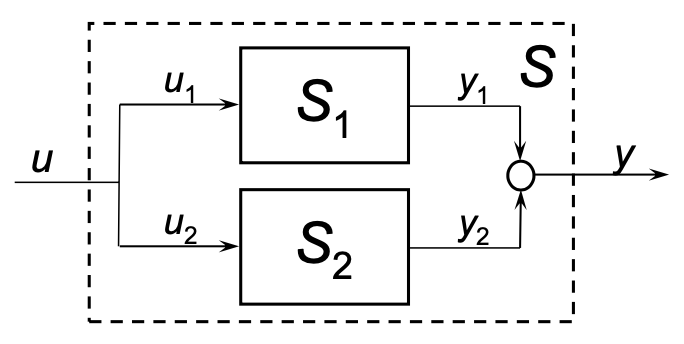
\includegraphics[scale=0.4]{immagini/parpass}
	\caption{The parallel of two passive systems is passive.}
	\label{fig:parpass}
\end{figure}
\begin{proof}
	If they are both dynamical systems, take as storage function the sum of the two storage functions. Then:\[	\dot{V}(x)=\dot{V}_1(x_1)+\dot{V}_2(x_2)\le y_1u_1+y_2u_2\le (y_1+y_2)u=yu\] If they are both static:\[0\le y_1u_1+y_2u_2=(y_1+y_2)u=yu\] If $S_1$ is static and $S_2$ dynamic \[\dot{V}(x)=\dot{V}_2(x_2)\le y_2u_2\le y_1u_1+y_2u_2\le (y_1+y_2)u=yu.\]
\end{proof}
\paragraph{Feedback}
\begin{figure}[H]
	\centering
	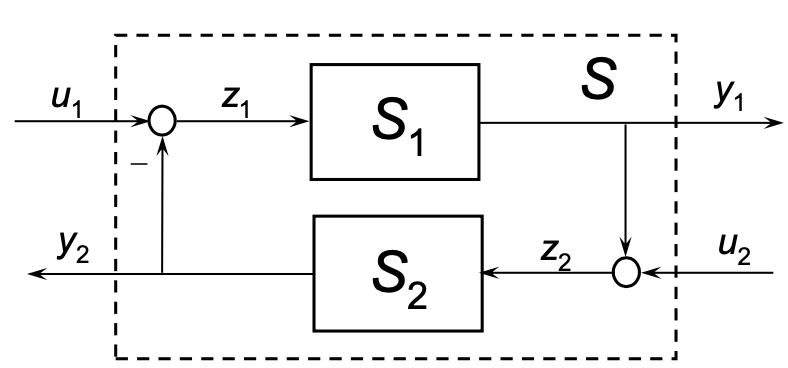
\includegraphics[scale=0.4]{immagini/feedpass}
	\caption{If two systems are passive, then, the resulting feedback systems with input $u_k$ and output $y_k$, k = 1,2, are passive.}
	\label{fig:feedpass}
\end{figure}
\begin{proof}
	If they are both dynamic, take as storage function the sum of the two storage functions. Then: \[\dot{V}(x)=\dot{V}_1(x_1)+\dot{V}_2(x_2)\le y_1z_1+y_2z_2\] where $y_1z_1+y_2z_2=y_1(u_1-y_2)+y_2(u_2+y_1)=y_1u_1+y_2u_2$.
	\\ If $S_1$ is static and $S_2$ dynamic, take as storage function that of $S_2$. Then: \[
	\dot{V}(x)=\dot{V}_2(x_2)\le y_2z_2\le y_1z_1 +y_2z_2
	\] where $y_1z_1+y_2z_2=y_1(u_1-y_2)+y_2(u_2+y_1)=y_1u_1+y_2u_2$.
\end{proof}

%%%%%% FINE CAPITOLO%%%%%%